\documentclass[a4paper, onecolumn, 12pt]{IEEEtran}
%\documentclass[draftcls, onecolumn, a4paper, twoside]{IEEEtran}


% These values get used many times, so it is easier to define then once here.
% Module code
\def\modulecode{ELI 220}
% Module name
\def\modulename{Linear Systems}
% Assessment title
\def\assessment{Practical 3}
\def\assessmenttitle{Realisation of analogue filters}
% Group number
\def\groupnumber{43}

% Student details: (Leave blank the last student(s) if your group has fewer people. The contributions MUST add up to 100%. Additional rows in the table on the title page can be commented out in titlepage.tex.)
% Details of the first student
\def\firststudentname{Emma Muller}
\def\firststudentnumber{24875882}
\def\firststudentcontribution{33.3}
% Details of the second student
\def\secondstudentname{Jan-Hendrik Brink}
\def\secondstudentnumber{23694956}
\def\secondstudentcontribution{33.3}
% Details of the third student
\def\thirdstudentname{Sean van Wyk}
\def\thirdstudentnumber{24606872}
\def\thirdstudentcontribution{33.3}


% Allows multi-line equations to be split over a number of pages.
\interdisplaylinepenalty=2500 


\usepackage{amsmath}
\usepackage{amssymb}
\usepackage{cite}
\usepackage{graphicx}
\usepackage{lastpage}
\usepackage{listings}
\usepackage{minted}
\usepackage{multirow}
\usepackage{paralist}
\usepackage{placeins}  % For \FloatBarrier
%\usepackage{rotfloat}
\usepackage{rotating}
\usepackage[tight,small]{subfigure}  % normalsize small footnotesize
\usepackage{tabularx}
\usepackage{tabulary}

% I prefer this to the default font.
\usepackage{newtxmath}
% \usepackage{newtxtext}
\renewcommand{\rmdefault}{ntxtlf} 
%https://tex.stackexchange.com/questions/347566/math-digits-are-rendered-in-cm-when-using-libertine-and-newtxmath-with-xelatex-i


% Set the page format up.
\usepackage{geometry}
\geometry{includefoot}
\geometry{paper=a4paper}
\geometry{left=25mm}
\geometry{right=25mm}
\geometry{top=25mm}
\geometry{bottom=20mm}
\geometry{headsep=10mm}
\geometry{footskip=10mm}
%\geometry{columnsep=4mm}


\usepackage[pdftex]{hyperref}
%\hypersetup{pdfborder={0 0 0.2}}
\usepackage{xcolor}
\definecolor{darkred}{rgb}{0.8,0,0}
\definecolor{darkgreen}{rgb}{0,0.45,0}
\definecolor{darkblue}{rgb}{0,0,0.3}
\hypersetup{colorlinks=True, citecolor=black, filecolor=black, linkcolor=black, urlcolor=black}

% Set the PDF properties of the document.
\hypersetup{%
  pdftitle={\modulecode-- \assessment: \assessmenttitle},
  pdfauthor={Group \groupnumber}}


\usepackage[acronym,nonumberlist,nopostdot,style=super]{glossaries}  % This must be after hyperref.

% Load the abbreviations.
% \loadglsentries{abbreviations}
% \makeglossaries

% % Format the abbreviations list.
% \renewenvironment{theglossary}%
% {%\vspace{-1em}%
% \begin{supertabular}{ @{} l p{\textwidth} }}% Added @{} here to get left justification.
% {\end{supertabular}}
% \renewcommand{\acronymname}{\vspace{-1.2em}}%Abbreviations}
% %\renewcommand{\glspostdescription}{}
% \renewcommand{\glsgroupskip}{}


\usepackage{fancyhdr}
% Set the page format up.
\def\pagenumberfooter{\thepage}
\fancypagestyle{plain}{%
  \fancyhf{}
  \lhead{}
  \rhead{}
  \lfoot{}
%  \cfoot{Confidential}
  \rfoot{\thepage}
  \renewcommand{\headrulewidth}{0pt}
  \renewcommand{\footrulewidth}{0pt}
}
\def\pagenumberfooter{\thepage}
\fancypagestyle{fancy}{%
  \fancyhf{}
  \lhead{}
  \rhead{}
  \lfoot{\modulecode~-- \assessment~-- Group \groupnumber}
%  \cfoot{Confidential}
  \rfoot{Page~\thepage~of~\pageref{LastPage}}
  \renewcommand{\headrulewidth}{0pt}
  \renewcommand{\footrulewidth}{0.5pt}
}


\hyphenation{mono-pulse}
\hyphenation{retro-directive}



% \renewcommand{\Re}{\mathrm{R\hspace{-0.09em}e\hspace{-0.08em}}}
% \renewcommand{\Im}{\mathrm{I\hspace{-0.07em}m\hspace{-0.08em}}}
% I prefer this to the default versions - feel free to disagree.
\usepackage[cal=boondoxo]{mathalfa}
\renewcommand{\Re}{\mathcal{R\hspace{-0.2em}e\hspace{-0.1em}}}
\renewcommand{\Im}{\mathcal{I\hspace{-0.25em}m\hspace{-0.15em}}}

\newlength{\equalswidth}
\settowidth{\equalswidth}{$ =~ $}
\newcommand{\eqsplitline}{\nonumber \\ & \hspace{\equalswidth}}
\newcommand{\eqsplitaligned}{\\ & \hspace{\equalswidth}}


%\setlength{\parindent}{0cm}
\setlength{\parskip}{0.3em plus 0.3em minus 0.3em}


%\def\today{27 March 2018}
% Get the Day Month Year format.
\def\today{%
  \number\day
  \space
  \ifcase\month\or January\or February\or March\or April\or May\or
  June\or July\or August\or September\or October\or November\or
  December\fi
  \space
  \number\year
}


% Allow large floats.
\renewcommand\topfraction{1}
\renewcommand\bottomfraction{0}
\renewcommand\textfraction{0}
\renewcommand\floatpagefraction{1}
\setcounter{topnumber}{10}
\setcounter{totalnumber}{10}


% Increase the figure caption font size.
\usepackage[font=normalsize]{caption}

% Deal with missing images which are not directly included in the repository
\newcommand{\noimage}{%
  \fbox{\parbox[t][0.3\textwidth][c]{0.48\textwidth}{\centering Image file is missing.}}
%  \setlength{\fboxsep}{-\fboxrule}%
%  \fbox{\phantom{\rule{10pt}{10pt}}File missing\phantom{\rule{10pt}{10pt}}}% Framed box
}
\let\includegraphicsoriginal\includegraphics
\renewcommand{\includegraphics}[2][width=\textwidth]
{%
  \IfFileExists{#2}
  {\includegraphicsoriginal[#1]{#2}}%
  {\noimage}%
%  {\fbox{\includegraphicsoriginal[#1]{drawings/gripen}\makebox[0pt]{File #2 is missing.}}}%
}

% Centred column in tabularx.
\newcolumntype{Y}{>{\centering\arraybackslash}X}


\begin{document}


% Try to keep text inside the right margin.
\sloppy


% The language used in the source-code listings.
\lstset{language=Python}
\lstset{numbers=left}
\lstset{basicstyle=\small}
\lstset{breaklines=true, breakatwhitespace=false}
\lstset{xleftmargin=7mm,linewidth=\textwidth,xrightmargin=7mm}

% Colours for code listings.
\definecolor{codegreen}{RGB}{0,200,0}
\definecolor{codepurple}{RGB}{220,0,220}
\definecolor{codecyan}{RGB}{0,200,200}

\lstset{keywordstyle=\color{blue}}%\bfseries}
\lstset{commentstyle=\color{codegreen}}%\itshape}
\lstset{stringstyle=\color{red}}

% Variables.
\lstset{classoffset=2,morekeywords={input, output, beat}, keywordstyle=\color{orange}, classoffset=0}
% Function names.
\lstset{classoffset=3,morekeywords={choice},keywordstyle=\color{codepurple},classoffset=0}
% Classes.
\lstset{classoffset=4,morekeywords={random},keywordstyle=\color{codecyan},classoffset=0}

\setminted{fontsize=\small,xleftmargin=7mm,xrightmargin=7mm, breaklines, breakanywhere, linenos}
\renewcommand\theFancyVerbLine{\small\arabic{FancyVerbLine}}

% Customise the reference format.
\bstctlcite{IEEEexample:BSTcontrol}


% Title page
% Title page

\newcolumntype{A}{>{\centering\arraybackslash}m{4cm}}
\newcolumntype{B}{>{\centering\arraybackslash}m{3.75cm}}
\newcolumntype{C}{>{\centering\arraybackslash}m{3.25cm}}

\begin{titlepage}
    \begin{center}

        \vspace*{2cm}
    
        % University Logo
        \includegraphics[width=0.6\textwidth]{plots/UPEBITlogo.jpg}\\[2.0cm]    
    	
        % Department Title
        \textsc{\LARGE\bfseries \modulecode}\\[1.0cm]
    	
        % Module Tile
        \textsc{\Large\bfseries \modulename}\\[0.75cm]
    
        % Assignment Title
        \textsc{\large\assessment:~\assessmenttitle}\\[0.5cm]
        
        %Group Number
        \textsc{\large Group \groupnumber}\\[1.0cm]
        
    		
        % Students/Contributors Table
        \begin{table}[h]
            \centering
            \normalsize
            \begin{tabularx}{\textwidth}{|A|C|B|C|}
                \hline
                \textbf{Name and Surname} & \textbf{Student Number} & \textbf{Signature} & \textbf{\% contribution} \\
                \hline
                \firststudentname   & \firststudentnumber   & \includegraphics[height=9mm]{plots/Emma.jpg} & \firststudentcontribution \\ 
                & & &   \\ \hline 
                \secondstudentname  & \secondstudentnumber  & \includegraphics[height=9mm]{plots/Jannie.png} & \secondstudentcontribution \\ 
                & & &   \\ \hline 
                \thirdstudentname   & \thirdstudentnumber   & \includegraphics[height=9mm]{plots/Sean.png} & \thirdstudentcontribution \\ 
                & & &   \\ \hline
            \end{tabularx}
        \end{table}
		
    \end{center}

  % Report Declaration
%   Comment this line out and uncomment the line below it in the \verb|report.tex| file to include the required declaration.
    \noindent By submitting this assignment we confirm that we have read and are aware of the University of Pretoria's policy on academic dishonesty and plagiarism and we declare that the work submitted in this assignment is our own as delimited by the mentioned policies. We explicitly declare that no parts of this assignment have been copied from current or previous students' work or any other sources (including the internet), whether copyrighted or not. We understand that we will be subjected to disciplinary actions should it be found that the work we submit here does not comply with the said policies.
	
	\vfill
    \begin{center}
		\large\today
    \end{center}

\end{titlepage}


%% Avoid expanding abbreviations.
%\glsunsetall
% Ensure that the abbreviations are expanded in the text.
% \glsresetall

% Table of Contents
\pagenumbering{roman}
\pagestyle{plain}
\setcounter{tocdepth}{2}
\addtocontents{toc}{\protect\thispagestyle{plain}}
\tableofcontents
\clearpage
\pagenumbering{arabic}
\setcounter{page}{1}
\pagestyle{fancy}


\section{Introduction}
\label{sec:introduction}

This practical focuses on the design, simulation and realisation of analogue active filters, which are fundamental components in signal processing and communication systems. The objective is to analyse and implement three specific filter types - namely, a Chebyshev low-pass filter, a Butterworth high-pass filter, and a minimal ripple band-pass filter - each designed with given frequency and attenuation specifications.

Through this practical, theoretical filter design principles are applied to derive transfer functions, determine component values, and construct corresponding circuits. Simulation and experimental methods are used to verify theoretical predictions by analysing the amplitude and phase responses of each filter, as well as evaluating key characteristics such s cut-off frequency, passband ripple, and roll-off rate.

Understanding the behaviour and performance differences between filter types is crucial in practical electronic design, as it allows engineers to select the most appropriate configuration for various applications requiring noise reduction, signal conditioning, or frequency selection. This practical therefore bridges theoretical knowledge of system analysis with hands-on circuit implementation, reinforcing key concepts in analogue signal processing.

\newpage
\section{Preparatory Work}
\label{sec:preparatory_work}

  \subsection{Chebyshev low-pass filter}
  \label{subsec:prep-low-pass} \strut
  The design specifications for the Chebyshev low-pass filter is that it must have a cut-off frequency of $4\,kHz$, a passband ripple of $1.0\,dB$ and a decay rate of $60\,dB/decade$. 
    
  The specification contains many valuable insights. It is known that for every $20\,dB/decade$ decay-rate the system increments in order \cite{lathi}. From this it is clear that this is a third order filter ($n=3$).

  The passband ripple of $1.0\,dB$ must be used to calculate the ripple-factor $\epsilon$. The ripple-factor is calculated using the following formula: 
  \begin{equation}
  \label{eqn:ripple_factor}
     A_p = 10\log(1+\epsilon^2)
  \end{equation}
  where $A_p$ is the band-pass ripple. Thus $A_p = 1\,dB$
  \begin{align*}
    1 &= 10\log(1+\epsilon^2) \\
    10^1 &= (1+\epsilon^2)^{10} \\
    \epsilon^2 &= 10^{\frac{1}{10}}-1 \\
    \epsilon^2 &= 0.2589.
  \end{align*}
  From \cite{carlson}, the following table entry for filter transfer function analysis can be found. 
    \begin{table}[H] 
      \centering 
      \caption{$1\,dB$ passband ripple Chebyshev filter coefficients from carlson}
      \begin{tabular}{|m{2cm}|m{2cm}|m{2cm}|m{2cm}|}
      \hline
        \multicolumn{4}{|c|}{$1\,dB$ Chebyshev passband ripple ($\epsilon^2=0.2589$)} \\ \hline
        n & $b_o$ & $b_1$ & $b_2$ \\ \hline 
        3 & 0.4913& 1.2384& 0.9883\\ \hline
      \end{tabular}
      
      \label{tbl:carlson_chebychev}
    \end{table}
    As shown by the specifications the filter is third order ($n=3$) and $\epsilon^2 = 0.2589$, thus the values for $b_0,b_1,b_2$ can be used from table (\ref{tbl:carlson_chebychev}).

    To realize the filter, the first step is to determine the transfer function. From \cite{carlson} when using table (\ref{tbl:carlson_chebychev}) the generic formula for the realizable transfer function is given by
    \begin{equation}
      H_{LN}(S_{LN}) = \frac{a_0}{b_o + b_1S_{LN}^{1} + ... + b_{n-1}S_{LN}^{n-1} + S_{LN}^{n}}
      \label{eqn:Hf_generic_norm}.
    \end{equation}
    It is important to note that $S_{LN}$ is normalized, meaning that the function is scaled to have a magnitude of $1$.
    To get the original transfer function the function must be denormalized. To denormalized according to \cite{carlson} when transforming from a normalized transfer function to a low-pass transfer function. The following relationship must be substituted into the normalized transfer fuction.
    \begin{equation}
      S_{LN} = \frac{s}{\omega_c}.
      \label{eqn:denorm}
    \end{equation}
    After the substitution 
    \begin{equation}
      H(s) = \frac{a_0}{b_o + b_1 \frac{s}{\omega_c}^{1} + ... + b_{n-1}\frac{s}{\omega_c}^{n-1} + \frac{s}{\omega_c}^{n}}.
      \label{eqn:Hf_generic_denorm}
    \end{equation}
    
    In order to simplify realization the expression is multiplied by $\frac{\omega_c^n}{\omega_c^n}$ :
    \begin{equation}
      H(s) = \frac{a_0}{b_o\omega_c^n + b_1s\omega_c^{n-1} + ... + b_{n-1}s^{n-1}\omega_c^{1} + s^n}
      \label{eqn:Hf_generic}
    \end{equation}
    With the generic transfer function (\ref{eqn:Hf_generic}) obtained, the specifications must be substituted into equation (\ref{eqn:Hf_generic}):
    \begin{align*}
      \omega_c = 4 kHz \, &= 8000\pi\,rad/s \\
      n &= 3     
    \end{align*}
    Since no specification for gain is provided, unity gain is assumed, so
    \begin{align*}
      G_m &= 1.
    \end{align*}
    From \cite{carlson} the variable $a_o$ can be calculated by substituting $s = 0$. 
    \begin{align*}
      H(0) &= G_m = \frac{a_o}{b_o} \\ 
      a_o &= b_o G_m = 0.4913 
    \end{align*}
    After substituting these values along with the values of $b$ from Table \ref{tbl:carlson_chebychev},
    \begin{equation}
      H(s) = \frac{7.7995 \times 10^{12}}{7.7995 \times 10^{12} + 782.24 \times 10^6 s + 24.8387 \times 10^3 s^2 + s^3},
      \label{eqn:Hs_subbed}
    \end{equation}
    where $s$ is $j2\pi f$. The Bode plot is provided in Figure (\ref{fig:chebyshev_theoretical}).

    \begin{figure}[H]
      \centering
      \includegraphics[width=0.8\textwidth]{figures/Chebyshev_theoretical.pdf}
      \caption{Magnitude response of the third-order Chebyshev low-pass filter}
      \label{fig:chebyshev_theoretical}
    \end{figure}

    To realize the filter the Sallen-key topology of Figure \ref{fig:chebyshev_filter} chosen \cite{sallenkey}. 
    
    \begin{figure}[H]
      \centering
      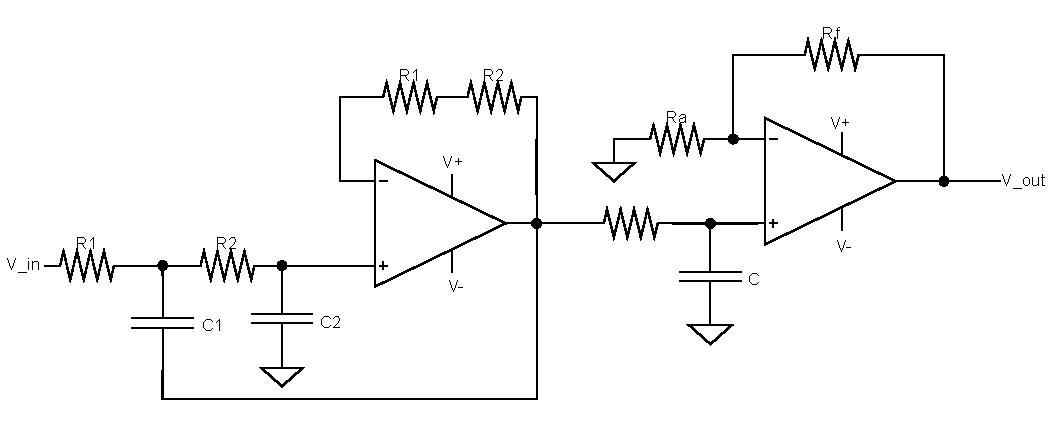
\includegraphics[width=0.8\textwidth]{figures/Chebyshev_sallen-key.pdf}
      \caption{Second-order low-pass Sallen-Key filter cascaded with first-order for Chebyshev filter}
      \label{fig:chebyshev_filter}
    \end{figure}

    In order to implement a third-order Chebyshev low-pass filter, the approach is to simply cascade a second and first order filter in series.

    Using the op-amp realization techniques presented in \cite{lathi} and \cite{carlson}, 
    \begin{equation}
      H_2(s) = \frac{1}{R_1R_2C_1C_2s^2 + (R_1 + R_2)C_2s + 1},
      \label{eqn:chebyshev_2nd}
    \end{equation}
    and
    \begin{equation}
      H_1(s) = \frac{1 + \frac{R_f}{R_a}}{RCs + 1}
      \label{eqn:chebyshev_1st}.
    \end{equation}
    It is known that due to the cascading property of op-amps the final third-order transfer function is
    \begin{equation}
      \nonumber
      H(s) = H_2(s) \times H_1(s)
    \end{equation}
    \begin{equation}
      H(s) = \frac{1}{R_1R_2C_1C_2s^2 + (R_1 + R_2)C_2s + 1} \times  \frac{1 + \frac{R_f}{R_a}}{RCs + 1}
      \label{eqn:Hs_fin}
    \end{equation}
    By factorising the denominator to get it in the form of a cascaded second and first order filter.
    \begin{equation}
      H(s) = \frac{1+\frac{R_f}{R_a}}{(R_1R_2C_1C_2s^2 + (R_1 + R_2)C_2s + 1)(RCs + 1)}
      \label{eqn:Hs_fin_fact}
    \end{equation}
    Applying the same factorization to equation (\ref{eqn:Hs_subbed}) yeilds
    \begin{equation}
      H(s) = \frac{7.7995 \times 10^{12}}{(s+12419.6)(s^2 + 12419.6s + 6.2799975 \times 10^8)}.
      \label{eqn:Hs_fin_1}
    \end{equation}
    Dividing by $12419.6$ to get the first order denominator in the correct form yeilds 
    \begin{equation}
            H(s) = \frac{627.99929 \times 10^{6}}{(80.51789 \times 10^{-6}s + 1)(s^2 + 12419.6s + 6.2799975 \times 10^8)}.
      \label{eqn:Hs_fin_2}
    \end{equation}
    Dividing by $6.279976 \times 10 ^ {8}$ to get the second order denominator in the correct form yeilds 
    \begin{equation}
      H(s) = \frac{1}{(80.51789 \times 10^{-6}s + 1)(1.5923 \times 10^{-9} s^2 + 19.7597 \times 10^{-6} s + 1)}.
      \label{eqn:Hs_fin_3}
    \end{equation}
    By comparing the equation (\ref{eqn:Hs_fin_fact}) to equation (\ref{eqn:Hs_fin_3}), it becomes apparent that
    \begin{align*}
      \frac{R_f}{R_a} &= 0 \\
      RC &= 80.5179 \times 10^{-6} \\ 
      R_1R_2C_1C_2 &= 1.5923573 \times 10^{-9} \\ 
      (R_1 + R_2)C_2 &= 19.7597 \times 10^{-6} .\\
      \label{eqn:Chebyshev_RC}
    \end{align*}
    Since there are 6 variables but only 3 equations, 3 of the variables can be any real value. These variables must be fixed to a convenient value, while electronic components become unreliable at extremely small or extremely large values. 
    For resistors a value between $1\,k\Omega$ and $100\,k\Omega$ is recommended, and for capacitors a value between $1\,nF$ and $1\,\mu F$.

    The values of $R_1 = R_2 = R = 10k \Omega$ were selected as this is ideal for a resistor and the calculated values for the capacitors were all reasonable.

    After substituting the fixed values for $R_1 , \, R_2$ and $R$ into the above equations, the following values for the circuit's capacitors were obtained:
    \begin{align*}
      RC = 80.517 \times 10^{-6} &\implies C = \frac{80.517 \times 10^{-6}}{R}, \\
      2RC_2 = 19.7597 \times 10^{-6} &\implies C_2 = \frac{19.7597 \times 10^{-6}}{2R}, \\ 
      R^2C_1C_2 = 1.5923574 \times 10^{-9} &\implies C_1 = \frac{1.5923 \times 10^{-9}}{R^2C_2}.
    \end{align*}
    Finally
    \begin{align*}
      R &= R_1 = R_2 = 10 k\,\Omega, \\ 
      C &= 8.05 nF, \\ 
      C_1 &= 16.1 nF, \\ 
      C_2 &= 0.988 nF.
    \end{align*}

    The filter is then simulated, as shown in Figures \ref{fig:chebyshev_spice} and \ref{fig:chebyshev_spice_sim}.
    \begin{figure}[H]
      \centering
      \includegraphics[width=1.0\textwidth]{figures/Chebyshev_spice.png}
      \caption{Chebyshev LTspice model with non-ideal op-amps}
      \label{fig:chebyshev_spice}
    \end{figure}

    \begin{figure}[H]
      \centering
      \includegraphics[width=0.9\textwidth]{figures/Chebyshev_sim_plot.png}
      \caption{Simulated frequency response of the Chebyshev low-pass filter.}
      \label{fig:chebyshev_spice_sim}
    \end{figure}


  \newpage
  \subsection{Butterworth high-pass filter}
  \label{subsec:prep-high-pass}

  The Butterworth response produces no ripple in the pass or stop band, resulting in a maximally flat filter response, but at the expense of a relatively wide transition band \cite{butterworth}. 

  The high-pass filter should have a cut-off frequency ($f_c$ or $\omega_c$) of $8\,kHz$ or $16000\pi\,rad/s$ with a $60\,dB/decade$ decay rate. This implies that the filter should be third-order, thus in order to find the transfer function the starting point in the Laplace domain is 
  \begin{equation}
    H_{LPN}(s) = \frac{K}{s^3 + 2s^2 + 2s 1},
  \end{equation}
  where $H_{LPN}$ refers to the normalised low-pass filter, and $K$ is the gain in $dB$ \cite{carlson}. Hereafter, to convert to the normalised high-pass form ($H_{HPN}$), $s$ was replaced by $\frac{1}{s}$ \cite{carlson}, so 
  \begin{equation}
    H_{HPN}(s) = \frac{Ks^3}{s^3 + 2s^2 + 2s 1}.
  \end{equation}
  This transformation is applied to invert the frequency axis, effectively swapping the low-frequency attenuation with high-frequency attenuation, thus converting the low-pass prototype into a high-pass response.
  For the desired $f_c$, $s \rightarrow \frac{s}{\omega_c}$ \cite{carlson}:
  \begin{align}
  \label{H_HP}
    H_{HP}(s) &= \frac{K(\frac{s}{\omega_c})^3}{(\frac{s}{\omega_c})^3 + 2(\frac{s}{\omega_c})^2 + 2(\frac{s}{\omega_c}) + 1} \nonumber \\
              &= \frac{Ks^3}{s^3 + 2\omega_cs^2 + 2\omega_c^2s +\omega_c^3},
  \end{align}
  where $\omega_c$ is $2\pi f_c$ and $s$ is $j2\pi f$. 

  For a third-order response, a first-order filter is cascaded via a buffer with a second-order circuit. This approach simplifies tuning, maintains stability, and allows independent adjustment of gain and $Q$-factor. For the first-order circuit, a passive RC filter will be used with transfer function
  \begin{equation}
  \label{H1_HP}
    H_1(s) = \frac{s}{s + \omega_c},
  \end{equation}
  where \cite{sallenkey}
  \begin{equation}
  \label{RC}
    \frac{1}{RC} = 2\pi f_c =\omega_c
  \end{equation}
  Furthermore, using the Sallen-Key (or KRC) configuration of Figure \ref{fig:sallenkey}, the second-order filter has the transfer function of 
  \begin{equation}
  \label{H2_HP}
    H_2(s) = \frac{Ks^2}{s^2 + \frac{\omega_c}{Q}s + \omega_c^2}.
  \end{equation}
  The Sallen-Key configuration is chosen due to its simplicity and suitability for implementing unity- or non-unity gain second-order active filters using a single operational amplifier.

  Multiplying equations (\ref{H1_HP}) and (\ref{H2_HP}) matches equation (\ref{H_HP}), implying that this design is valid.

  \begin{figure}[h]
    \centering
    \includegraphics[width=0.8\textwidth]{figures/sallenkey.drawio.png}
    \caption{General Sallen-Key second-order high-pass filter configuration}
    \label{fig:sallenkey}
  \end{figure}

  For simplicity, it is assumed that all resistance and capacitance values are equal. However, to ensure that $f_c$ sits at the $-3\,dB$ point, a $Q$ (selectivity) value of 1.0 needs to be used \cite{carlson}, then by 
  \begin{align}
    Q &= \frac{1}{(1-K)\sqrt{\frac{R_2C_2}{R_1C_1}} + \sqrt{\frac{R_2C_2}{R_1C_1}} + \sqrt{\frac{R_1C_1}{R_2C_2}}} \nonumber \\
      &= \frac{1}{(1-K) + 1 + 1},
  \end{align}
  $K$ is calculated to be 2 with
  \begin{equation}
    K = 1 + \frac{R_B}{R_A}.
  \end{equation} 
  For a Butterworth response, all poles are equally spaced on the unity circle, yielding a damping ratio corresponding to $Q=1.0$ for the second-order stage. This ensures a maximally flat passband and no peaking near the cut-off frequency.

  Using equation (\ref{RC}), $RC$ is calculated to be $1.9894367 \times 10^{-5}$. This ratio is then used to determine multiple possible capacitor and resistor values, but finally $20\,k\Omega$ and $1\,nF$ was chosen in order to ensure sufficient capacitance and efficient power usage. Assuming $R_A\,=\,R_B$, a large resistance of $100\,k\Omega$ was chosen for each. The final circuit design is shown in Figure \ref{fig:highpass}.

  Furthermore, the final transfer function is then 
  \begin{equation}
  \label{H_HP(s)_final}
    H_{HP}(s) = \frac{2s^3}{s^3 + 100530.96s^2 + 5.06\times10^9s + 1.27\times10^{14}},
  \end{equation}
  or, expressed in terms of $f$
  \begin{equation}
  \label{H_HP(f)_final}
    H_{HP}(f) = \frac{-j496.1f^3}{-j248.05f^3 - 3.9688\times10^6f^2 + j3.179\times10^{10}f + 1.27\times10^{14}}.
  \end{equation}
  This result is shown in Figure \ref{fig:highpass_hf}. With a pass-band gain of $6\,dB$, $f_c$ is now at $3\,dB$ ($-3\,dB$ relative to $6\,dB$).

  \begin{figure}[h]
    \centering
    \includegraphics[width=0.8\textwidth]{plots/matlab_highpass.pdf}
    \caption{Plot of $H(f)$ for the high-pass filter}
    \label{fig:highpass_hf} 
  \end{figure}

  The resulting Bode plot in Figure \ref{fig:highpass_hf} confirms the expected Butterworth characteristics - a smooth passband with no ripple, a $-3\,dB$ attenuation at $f_c = 8\,kHz$, and a roll-off rate of approximately $60\,dB/decade$ (third-order response).

  In addition to the amplitude response, the phase response was also plotted in Figure \ref{fig:highpass_hf}. The phase begins at approximately $-90^\circ$ at low-frequencies, characteristic of a first-order high-pass response. As the frequency increases through the cut-off region, the cumulative phase shift increases due to the additional second-order stage, reaching approximately $-180^\circ$ near $f_c$, ultimately approaching $-270^\circ$ at high-frequencies. This behavior is also consistent with the expected third-order Butterworth response, which exhibits a smooth and monotonic phase transition \cite{carlson}.

  \begin{figure}[h]
    \centering
    \includegraphics[width=0.8\textwidth]{figures/highpass_final.drawio.png}
    \caption{Circuit for the Butterworth high-pass filter}
    \label{fig:highpass}
  \end{figure}

  To further verify the design the circuit in Figure \ref{fig:highpass}, was simulated using a frequency sweep from $1\,Hz$ to $1\,MHz$ and a $1\,V$ AC source in LTSpice. The resulting plot is shown in Figure \ref{fig:HP_sim}. It is clear that the design is theoretically correct.

  \begin{figure}[h]
    \centering
    \includegraphics[width=\textwidth]{figures/highpass_ltspice.pdf}
    \caption{Simulated response of the high-pass filter}
    \label{fig:HP_sim}
  \end{figure}
  

  \subsection{Minimal ripple band-pass filter}
  \label{subsec:prep-band-pass}
  
  %%%%% DRAFT DRAFT DRAFT DRAFT DRAFT %%%%% NOT FINAL %%%%% 0 EDITING DONE SO FAR %%%%% DO NOT JUDGE YET PLEASE %%%%%
A key requirement of the band-pass filter is minimal output ripple. This excludes higher-order Chebyshev type responses. Another requirement is a roll off rate of $40\,dB/decade$ with a pass-band of $8 - 80\,kHz$ ($f_h$ the higher cutoff frequency of $80\,kHz$ and $f_l$ the lower cutoff frequency of $8\,kHz$). The design of a second-order Chebyshev was chosen for its faster more precise roll off rate and its minimal output ripple.

The following equation was obtained to find the centre frequency of the band-pass filter \cite{lancaster1996active},

\begin{equation}
  \label{CentreFreq}
  f_c = \sqrt{f_l \times f_h} \nonumber 
\end{equation}

Substituting $f_l$ and $f_h$ into equation (\ref{CentreFreq}) an $f_c$ of $25.3\,kHz$ is obtained.

To determine the Q-factor  the following equation is used from \cite{lancaster1996active},

\begin{equation}
  \label{QFactor}
  Q = \frac{f_c}{f_h - f_l}
\end{equation}

and a Q-factor of 0.35 is obtained. This classifies the filter as a wideband filter \cite{lancaster1996active}. For wideband filters, where Q is less than 1, the design can be simplified by cascading two separate filters in series, namely a high-pass and low-pass filter (feeding the output of one filter into the input of the next).

The Sallen-Key filter topology was chosen due to being well-documented and simple. Figure \ref{fig:sallenkey} shows the circuit diagram for a high-pass Sallen-Key segment.

The time domain equation \ref{Freq_Block}, that relates the values of R and C is obtained from \cite{lancaster1996active}. $R_f$ is chosen to be $10\,k\Omega$ as advised in \cite{lancaster1996active}. 
%yes perfect dankie
\begin{equation}
  F_b = \frac{1}{2\pi R C}
  \label{Freq_Block}
\end{equation}

Choosing $C = 100\,nF$ and substituting $F_h = F_b = 80\,kHz$ into the equation, a resistance value of $R = 200\,\Omega$ is obtained and a standard $240\,\Omega$ resistor is chosen. This should result in only a negligible shift in the cutoff frequency.

Following the high-pass stage, a low-pass filter with a cutoff frequency of $8\,kHz$ is designed using the circuit topology in Figure (\ref{fig:LP_Salenkey}).

\begin{figure}[H]
  \centering
  \includegraphics[width=\textwidth]{figures/LPSallenkey.pdf}
  \caption{Low-pass Sallen-Key filter circuit topology}
  \label{fig:LP_Salenkey}
\end{figure}

Again a $R_f$ of $10\,k\Omega$ with $C = 1\,nF$ is used. This is substituted into equation (\ref{Freq_Block}) with $F_b = F_l = 8\,kHz$ yielding a resistance of $R = 2\,k\Omega$.

Placing all the calculated components into the final filter design results in the circuit of Figure \ref{fig:BP_design}.

\begin{figure}[H]
  \centering
  \includegraphics[width=\textwidth]{figures/BPfilter.pdf}
  \caption{Cascaded Band-pass filter with values}
  \label{fig:BP_design}
\end{figure}

Simulating this circuit, results in Figure \ref{fig:BP_sim}.

\begin{figure}[H]
  \centering
  \includegraphics[width=\textwidth]{figures/SimBP.pdf}
  \caption{Simulated response of Band-pass filter in LTSpice}
  \label{fig:BP_sim}
\end{figure}

From the simulated response the minimal output ripple can be observed, only containing one peak at the latter frequencies of the response, but has a nearly perfect flat response elsewhere and a fast roll-off rate as required.

Converting this simulation into a transfer function in the Laplace domain is done similarly to the method outlined in \ref{subsec:prep-low-pass}. Equation \ref{eqn:Hf_generic_denorm} is transformed to a band-pass function by using the following conversion equation,

\begin{equation}
  s = \frac{s^2 + \omega_0^2}{W_s},
  \label{eqn:BPconversion}
\end{equation}

where $\omega_0 = 2\pi f_c$, and $\omega_0 = 159\,k\,rad/s$. Furthemore, $W_s = 2\pi(f_h-f_l)$ which is equal to $W_s = 452\,k\,rad/s$. After these substitutions equation \ref{eqn:Hf_generic_denorm} is

\begin{equation}
  H(s) = \frac{2.046 \times 10^{11} s^2}{s^4 + 516.4\times 10^3 s^3 + 2.552 \times 10^{11} s^2 + 1.616 \times 10^{16} s + 6.384 \times 10^{20}}.
  \label{BPTransfer}
\end{equation}

Plotting (\ref{BPTransfer}) in MatLab delivered the following bode plot.

\begin{figure}[H]
  \centering
  \includegraphics[width=\textwidth]{figures/BPTransFuncUPDATED.pdf}
  \caption{Transfer function of Band-pass filter}
  \label{fig:BPTransfer_sim}
\end{figure}

From Figure (\ref{fig:BPTransfer_sim}) it is evident that the decay-rate and cutoff frequencies are as expected and correlate nicely to Figure [\ref{fig:BP_sim}].

\newpage
\section{Practical Results}
\label{sec:practical_results}

  For all filters an AC source with $1\,V$ amplitude was used as input, in conjunction with a sinusoidal frequency sweep from the signal generator. The theoretically perfect component values did not exist in standard components so close enough alternatives were used.
  

  \subsection{Chebyshev low-pass filter}
  \label{subsec:prac-low-pass}

  The circuit outlined in Figure \ref{fig:chebyshev_filter} was physically implemented using breadboards and discrete components.
  All resistors were implemented using standard $10\,k\Omega$ resistors.
  For capacitor $C$ a value of $8.2\,nF$ was chosen. Capacitor $C_1$ is implemented using a parallel connection of two $8.2\,nF$ capacitors to get n value of $16.4\,nF$. For capacitor $C_2$ a value of $1\,nF$ was chosen.

  The laboratory signal generator was used to generate a sine wave frequency sweep from $1\,Hz$ to $50\,kHz$ over $1\,minute$. Using the oscilloscope's built-in FFT function, Figure \ref{fig:LP_FFT} was captured.

  \begin{figure}[H]
    \centering
    \includegraphics[width=0.8\textwidth]{figures/LP_FFT.PNG}
    \caption{FFT of the low-pass Chebyshev filter}
    \label{fig:LP_FFT}
  \end{figure}

  The ripple of the Chebyshev filter is clearly visible. The $4\,kHz$ cutoff frequency is very accurate as the FFT is at $-2.5\,dB$ at $4\,kHz$. The pass-band ripple is slightly higher than expected at $1.15\,dB$. The roll-off rate is difficult to determine per decade, since there seem to be a noise band that obscures the reponse after $15\,kHz$, however the roll-off rate per octave is $18.6\,dB$ which attenuates slightly faster than expected.

  The low-pass Chebyshev filter has a response within the acceptable margin of error from that displayed in the theoretical simulations and calculations.

  \subsection{Butterworth high-pass filter}
  \label{subsec:prac-high-pass}

  The circuit of Figure \ref{fig:highpass} was constructed on a breadboard and a sinusoidal frequency sweep from $1\,Hz$ to $40\,kHz$ was performed. The resulting FFT is shown in Figure \ref{fig:HP_FFT}.

  \begin{figure}[h]
    \centering
    \includegraphics[width=0.8\textwidth]{figures/HP_FFT.PNG}
    \caption{FFT of the high-pass filter}
    \label{fig:HP_FFT}
  \end{figure}

  Overall, the shape of the frequency response is as expected. The cut-off frequency, however, is now at approximately $9.60\,dB$, which is also unexpected. The decay-rate, however, remains approximately $60\,dB/decade$. 

  \subsection{Minimal ripple band-pass filter}
  \label{subsec:prac-band-pass}

The circuit seen in Figure~\ref{fig:BP_design} was constructed on a breadboard and a sinusoidal frequency sweep from $1$ to $500~\text{kHz}$ was performed. The resulting FFT is shown in Figure~\ref{fig:BP_FFT}.

\begin{figure}[h]
  \centering
  \includegraphics[width=0.8\textwidth]{figures/BP_FFT.PNG}
  \caption{FFT of the band-pass filter}
  \label{fig:BP_FFT}
\end{figure}

The frequency response exhibits the expected bandpass characteristics. However, notable differences exist between the simulation and experimental results - the lower passband cutoff is shifted lower by approximately $2~\text{kHz}$, while the upper passband cutoff is shifted higher by approximately $10~\text{kHz}$. Several factors may contribute to this discrepancy, as discussed in Section~\ref{sec:discussion}. The measured roll-off rate of $36~\text{dB/decade}$ closely matches the expected value.

\newpage
\section{Discussion}
\label{sec:discussion}

\subsection{Chebyshev low-pass filter}
The practical result nearly matches that of the simulated and theoretical results. The deviations observed in the practical test could have many reasons, one of which is likely the not perfectly accurate components used to construct the filter as an $8.2\,nF$ capacitor was used for $C$ instead of the theoretical $8.05\,nF$ capacitor. The influences of parasitic capacitance due to the non-ideal nature of a bread-board and the long parallel conductive rails by which the bread-board functions would also have infuenced the final results. It is also apparent that there is a low-amplitude noise band that obfuscates the stop-band.

%=======JANNIE ADD JOU DISCUSSION BO HIERDIE====================

\subsection{Butterworth high-pass filter}
Overall the experimental results confirm that the circuit behaves as a third-order Butterworth high-pass filter, with a few undesirable results in the FFT of Figure \ref{fig:HP_FFT}. The position of the cut-off frequency (or change in gain from $6\,dB$ to approximately $12.6\,dB$) could be due to component tolerances and environmental factors. Potentiometers could possibly reduce this discrepancy. 

At frequencies less than $800\,Hz$, a sharp peak is seen. This could be due to the large increase in the gain from theoretical to experimental results. The minor irregularities in the lower-frequency region of the FFT may be caused by noise pickup and the frequency resolution of the oscilloscope's FFT function.

%=======SEAN ADD JOU DISCUSSION ONDER HIERDIE===================%

\subsection{Minimal ripple bandpass filter}
The design and implementation of the second order band-pass filter delivered results that mostly matched expectations, with some notable differences. The lower cutoff frequency shifted nearly $2~\text{kHz}$ earlier (from $8~\text{kHz}$ to approximately $6~\text{kHz}$), while the upper cutoff frequency shifted nearly $10~\text{kHz}$ later (from $80~\text{kHz}$ to approximately $90~\text{kHz}$). There is a myriad of reasons that might explain why this is. The parasitic capacitance of the breadboard might have an influence or the decision to use $240~\Omega$ resistors in the high-pass segment instead of the theoretical $200~\Omega$.

Another difference is the roll-off rate of the practical filter that matched the simulation much closer than expected with a rate of $36~\text{dB/decade}$ compared to the designed $40~\text{dB/decade}$. Lastly the passband ripple that was clear in the simulation was imperceptible in the physical implementation. This confirmed the educated guess that a lower order Chebyshev filter can have minimal ripple as required.

%===============================================================
\subsection{Comparison between Chebyshev and Butterworth filter types}
Due to the ripple in its passband, a Chebyshev filter may be undesirable in some applications, but the fast transition is ideal in situations where maximum signal suppression is required. This makes a Chebyshev ideal for use in radio communication systems, audio systems and instrumentation \cite{chebyshev_butterworth_comparison}.

The Butterworth filter is characterised by its smooth but slow transition. These filters are predictable and may be more forgiving to component tolerances, but their slow decay-rate is a notable trade-off. These filters are suitable for applications that prioritise smooth frequency response over a sharp drop-off, perfect for applications in audio systems, medical imaging and telecommunications \cite{chebyshev_butterworth_comparison}. In order to achieve a better selectivity factor (similar to the Chebyshev) a higher-order circuit may be required, creating a more complex implementation. 


\newpage
\section{Conclusion}
\label{sec:conclusion}

This practical assignment successfully achieved its primary goals by guiding the design, simulation, and analysis of three distinct analogue filters: a Chebyshev low-pass filter, a Butterworth high-pass filter, and a minimal ripple band-pass filter.

The preparatory work established a solid theoretical foundation, where the transfer functions for each filter were derived analytically and their frequency responses were visualized using computational tools. This was followed by the design and simulation of corresponding circuits, which provided a predicted performance benchmark. The experimental simulation work then served to validate these theoretical models.

The results demonstrated a strong correlation between the theoretical predictions and the simulated experimental outcomes. Key filter characteristics—including the cut-off frequencies of approximately 4 kHz and 8 kHz for the low-pass and high-pass filters, respectively, the 8 kHz to 80 kHz passband for the band-pass filter, and the target decay rates—were clearly observed and measured. Notably, the distinct 1.0 dB passband ripple of the Chebyshev filter was visible, confirming its expected behaviour compared to the maximally flat response of the Butterworth filter.

Minor discrepancies between the theoretical and practical results, such as slight shifts in cut-off frequencies or deviations in the steepness of the roll-off, can be attributed to factors like component tolerances and non-ideal op-amp behaviour in the simulation models. The comparative analysis highlighted the fundamental trade-offs in filter design: the Chebyshev filter provides a steeper roll-off at the expense of passband ripple, while the Butterworth filter offers a smooth passband with a more gradual transition.

In summary, this practical not only reinforced the fundamental concepts of active filter design but also provided valuable hands-on experience in translating theoretical transfer functions into functional circuits and critically evaluating their performance. All the primary objectives of the practical were successfully met.

\newpage

% Make the reference font the same size as the rest of the text.
\IEEEtriggercmd{\normalsize}
\IEEEtriggeratref{1}

\bibliographystyle{IEEEtran}%
\bibliography{references}%

%\clearpage
\FloatBarrier


% Use for only one appendix (no titles necessary and no appendix numbers).
%\appendix
% Use for multiple appendices (with appendix numbers).
\newpage
\appendices

\section{Code}
\label{app:code}

\subsubsection{Python script to generate graph of the Chebyshev low-pass filter}
\label{sec:code_chebychev}
  \begin{mdframed}
    \inputminted{python}{./code/practical_3.py}
  \end{mdframed}

\subsubsection{MATLAB script to generate the Bode plot for the Butterworth high-pass filter}
\begin{mdframed}
  \inputminted{Matlab}{./code/Hf.m}
\end{mdframed}

\subsubsection{MATLAB script to generate the Bode plot for the Chebyshev band-pass filter}
\begin{mdframed}
  \inputminted{Matlab}{./code/BP_Filter.m}
\end{mdframed}



\end{document}
